\documentclass[11pt,a4paper]{article}
\usepackage[margin=1in]{geometry}
\usepackage{amsmath,amssymb}
\usepackage{bm}
\usepackage{tikz}

\begin{document}

\noindent\textbf{Vector diagram:}

\begin{center}
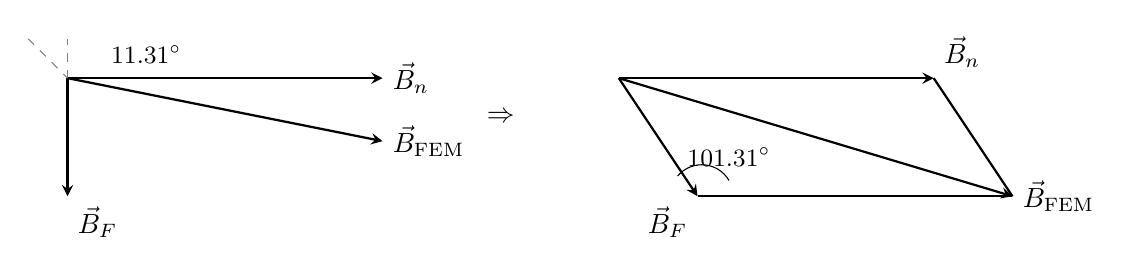
\begin{tikzpicture}[scale=1.0, >=stealth]
% ===== LEFT diagram =====
% B_n horizontal
\draw[->, thick] (0,0) -- (4,0) node[right]{$\vec{B}_n$};
% B_FEM slightly down-right (11.31 degrees from B_n)
\draw[->, thick] (0,0) -- (4,-0.8) node[right]{$\vec{B}_{\text{FEM}}$};
% B_F vertical down
\draw[->, thick] (0,0) -- (0,-1.5) node[below right]{$\vec{B}_F$};
% Angle label
\node at (1.0, 0.3) {\small $11.31^\circ$};
% Dashed extension lines
\draw[dashed, gray] (-0.5,0.5) -- (0,0);
\draw[dashed, gray] (0,0) -- (0,0.5);

% Arrow between
\node at (5.5, -0.5) {$\Rightarrow$};

% ===== RIGHT diagram (parallelogram) =====
% Vertices of parallelogram:
%   A = (7, 0)    top-left (origin)
%   B = (11, 0)   top-right (B_n end)
%   C = (12, -1.5) bottom-right (B_FEM end)
%   D = (8, -1.5)  bottom-left (B_F end)
\coordinate (A) at (7, 0);
\coordinate (B) at (11, 0);
\coordinate (C) at (12, -1.5);
\coordinate (D) at (8, -1.5);

% B_n (top edge)
\draw[->, thick] (A) -- (B) node[above right]{$\vec{B}_n$};
% B_FEM (diagonal)
\draw[->, thick] (A) -- (C) node[right]{$\vec{B}_{\text{FEM}}$};
% B_F (bottom edge, A to D)
\draw[->, thick] (A) -- (D) node[below left]{$\vec{B}_F$};
% Complete the parallelogram (light lines)
\draw[thick] (B) -- (C);
\draw[thick] (D) -- (C);

% Angle 101.31 between B_F and B_FEM (at vertex D... no, at vertex A between B_F direction and B_FEM)
% Actually from the photo, the 101.31 angle is at vertex D (bottom-left) between DA (going up) and DC (going right)
% Or at vertex A between B_F (going down-right) and B_FEM (going right)
% Looking again: the angle is marked at the BOTTOM, near B_F label, between B_F and B_FEM
\draw (8.4, -1.3) arc[start angle=30, end angle=140, radius=0.4];
\node at (8.4, -1.0) {\small $101.31^\circ$};
\end{tikzpicture}
\end{center}

\bigskip

\noindent By the Law of Cosines:
\begin{equation*}
\cos(101.31^\circ) = \frac{\vec{B}_n^{\,2} + \vec{B}_F^{\,2} - \vec{B}_{\text{FEM}}^{\,2}}{2 \cdot \vec{B}_n \cdot \vec{B}_F}
= \frac{135.98^2 + \vec{B}_F^{\,2} - 136.4^2}{2 \cdot 135.98 \cdot \vec{B}_F}
\end{equation*}

\bigskip

\begin{equation*}
\Rightarrow \boxed{\vec{B}_F = 2.065 \ \mathrm{mT}}
\end{equation*}

\end{document}
